\chapter{Physically Based Rendering}
\label{chap:pbr}

\acl{PBR} beschreibt ein relativ neues Oberflächenmaterial- und Beleuchtungskonzept in der Spieleindustrie. Es basiert auf dem von Disney vorgestelltem Beleuchtungsmodell \parencite{Burley2012} oder \parencite{Gotanda}. Während Disney ein festes Beleuchtungsmodell entwickelte, gibt \ac{PBR} kein festes Regelwerk vor und ist daher vielmehr als ein Paradigma zu verstehen, das erlaubt die Wechselwirkung von Licht, Oberflächen und Betrachter allgemeingültig und akkurat zu simulieren \parencite[Kapitel 1]{Rousiers2014}. Es führt dabei auch kein weiteres Beleuchtungsmodell ein, sondern lässt sich mit unterschiedlichen Approximationen der BRDF nutzen. Nicht desto trotz bedeutet die Umstellung auf ein \ac{PBR} Verfahren eine komplette Umstellung der Produktions- und Renderpipeline. In diesem Kapitel geben wir einen kurzen Überblick über die Prinzipien von \ac{PBR} und Beweggründe, warum es sich lohnen könnte, dieses Konzept praktisch umzusetzen.

\section{Gründe für \ac{PBR}}
\label{sec:pbr-warum}

Die Fähigkeiten einer Grafikengine werden oft daran beurteilt wie plausibel und realistisch die synthetisierten Bilder wirken. Um entsprechende Bilder in Echtzeit rendern zu können, müssen Kompromisse eingegangen werden. Während offline Renderverfahren mehr Freiheiten haben sich dem Realismus anzunähern, sorgen die Approximationen der Ad-hoc Shading Modelle \parencite{Martinez2010} oft für Probleme.

Der Künstler produziert 3D Modelle oft in einer von der Echtzeitengine isolierten Software Umgebung die ihre eigenen realistischem Beleuchtungsmodell besitzen. In den Ad-Hoc Modellen  gibt in der Regel nur wenige Oberflächenparameter, die zusätzlich in keinem physikalischen Zusammenhang zueinader gesetzt werden. Oft lassen sich die unterschiedlichen Parameter gar nicht direkt in einen physikalen Zusammenhang setzen, da sie überwiegend unabhängig von einander eingeführt wurden. Zum Beispiel wird das Ob und Wie Oberflächen die Umgebung spiegeln oft unabhängig vom sonstigen Lichtreflexionsverhalten (z.B. Spekularer Wert) gesteuert. Dies führt oft zu physikalisch inkorrekten Beleuchtungen. Dies führt zu vielen Spezialfällen und vielen Iterationen auf Künstlerseite, bis das Objekt mit der gewünschten Oberflächenbeleuchtung in der speziellen Szeneneinstellung dargestellt wird. Ändern sich die Beleuchtungsparameter und Szeneneinstellungen sind die mühsam justierten Einstellungen wieder hinfällig. 

Mit \ac{PBR} werden die klassischen Ad-hoc zusammengestellten Beleuchtungsmodelle verworfen, damit Beleuchtungsmodelle entworfen werden können, deren Parameter sich in einem physikalisch sinnvollem Zusammenhang setzen lassen. Nur dadurch lassen sich Spezialfälle vermeiden und es lässt sich eine visuelle Konsistenz herstellen. Visuelle Konsistenz bedeutet in diesem Zusammhang, dass sich einmal konfigurierte Oberflächeneigenschaften in unterschiedlichen Beleuchtungssituationen realistisch plausibel und verhersagbar verhalten. 

Dies wird dadurch erreicht, dass die Eigenschaften der Lichtquellen, die Oberflächeneingenschaften und der Betrachter von einander entkoppelt werden. Ziel ist meist ein einheitliches Shading Modell zu entwickeln, das für alle möglichen Szeneneinstellungen geeignet ist.

\section{Theoretische Grundlagen}
\label{sec:pbr-grundlagen}

\begin{table}
\centering
\begin{tabular}{c l}
\hline
	$\mathbf V$ & Richtungsvektor zum Betrachter \\
	$\mathbf L$ & Richtungsvektor zur Lichtquelle \\
	$\mathbf N$ & Oberflächennormale \\
	$m$ 	 	& Rauheitswert der Oberfläche (\textit{Roughness}) \\
 	$f$ 		& \textit{BRDF} \\
	$f_d$ 		& Diffuser Term der \textit{BRDF} \\
	$f_s$ 		& Spekularer Term der \textit{BRDF}\\
\hline
\end{tabular}
\caption[Notation \textit{BRDF}]{Notation}
\label{tab:pbr-notation}
\end{table}

Wie für die meisten Beleuchtungsmodelle bildet die \ac{BRDF} auch für das Konzept \ac{PBR} die theoretische Grundlage. Die \ac{BRDF} beschreibt das Reflexionsverhalten von Oberflächen. Sie lässt sich aus den zwei getrennten Termen für die diffuse $f_d$ und spekulare Reflexion $f_s$ zusammensetzen \parencite[Kapitel 3.1.2, Seite 7]{Rousiers2014}. So lassen sich beide Terme getrennt von einander betrachten sowie unterschiedliche Modelle und spezialisierte Approximationen finden. Im folgenden werden wir die in \fref{tab:pbr-notation} genannte Notation verwenden.

\begin{align}
	\label{eq:brdf-dekonstruiert}
	% \caption{Dekonstruierte BRDF}
	f(\mathbf V,\mathbf L) &= f_d(\mathbf V,\mathbf L) + f_s(\mathbf V,\mathbf L)\\
\end{align}


\subsection[Spekulares Reflexionsverhalten]{Spekulares Reflexionsverhalten $f_r$}
Das Reflexionsverhalten wird in der Realität wesentlich von der Oberflächenbeschaffenheit des Materials bestimmt. Polierte Oberflächen spiegeln, im Gegensatz zu rauhen Oberflächen, die Umgebung und erhalten Glanzlichter bei direkter Beleuchtung. Irreguläre rauhe Oberflächen streuen das einfallende Licht ungleichmäßig in alle Richtungen. Reguläre glatte Oberflächen reflektieren das einfallene Licht über die Fläche betrachtet gleichförmig (\warn{isotropic? nicht ganz}).

\begin{figure}
	\label{fig:microfacet}
	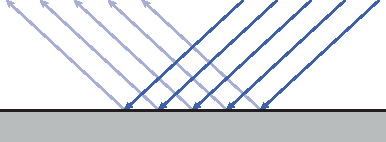
\includegraphics[width=.5\textwidth]{img/roughness0}
	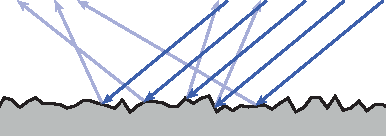
\includegraphics[width=.5\textwidth]{img/roughness1}
	\caption{links: $m = 0$; rechts $m = 1$}
\end{figure}

Ein realistisches Reflexionsmodell muss diese Oberflächenbeschaffenheit berücksichtigen. In Echtzeitverfahren ist es nicht praktikabel die mikroskopischen Unebenheiten, genannt \textit{Microfacetten oder Microfecets} (siehe \fref{fig:microfacet}), exakt zu berechenen. Entsprechend wurden einige approximierende Microfacet Modelle entwickelt, die die Interaktion des Lichts mit den Facetten realistisch abbilden können. Ein oft verwendetes Microfacet Modell ist die Cook-Torrance Modell \parencite{Cook1981} welches in \fref{eq:cook-torrance-model} dargestellt wird \parencite[Kapitel 6.9.2, Seite 194]{Lengyel2003}.

\begin{align}
	\label{eq:cook-torrance-model}
	% \caption{Cook-Torrance Illumination}
	f_s(\mathbf V,\mathbf L) = \mathcal{F}(\mathbf V,\mathbf L)\frac{D(\mathbf V,\mathbf L)G(\mathbf V,\mathbf L)}{\pi(\mathbf N \cdot \mathbf V)(\mathbf N \cdot \mathbf L)}
\end{align}

\section{Umsetzung}
\label{sec:pbr-umsetzung}

bla

\section{Wo wird es eingesetzt?}
\label{sec:pbr-wo}
Inzwischen wird das Verfahren in allen großen Spieleengines eingesetzt: CryEngine \parencite{Schulz2014}, Unreal Engine 4 \parencite{Martin2012}, Frostbite \parencite{Lagarde2014} und der Engine hinter den Call of Duty Titeln \parencite{Lazarov2011}.
